%
% Optional reading
%

\begin{frame}[plain,c]
\begin{center}
{\Huge \bf Optional reading for Lecture \thislecture}
\end{center}
\end{frame}

% ------------------------------------------------------------------------------

%
% Worked example :
%

{
\problemslide

\begin{frame}{Worked example: Exploiting the superposition principle}

  \begin{blockexmplque}{Question}
    A nonconductive solid sphere has a uniform volume charge density $\rho$.\\
    \vspace{0.1cm}
    Let $\vec{r}$ be the vector from the centre of the sphere to a general point
    $P$ within the sphere. As you should be able to easily confirm,
    the electric field $\vec{E}$ at a point $\vec{r}$  within the sphere is
    given by $\vec{E}(\vec{r}) = \rho \vec{r}/(3\epsilon_0)$.\\
    \vspace{0.1cm}
    If a spherical cavity is hollowed out of the sphere, as shown below,
    using superposition concepts, show that the electric field at all points
    within the cavity is uniform and equal to
    $\vec{E}(\vec{r})=\rho \vec{a}/(3\epsilon_0)$
    where $\vec{a}$ is the position vector
    from the centre of the sphere to the centre of the cavity.\\
    \begin{center}
      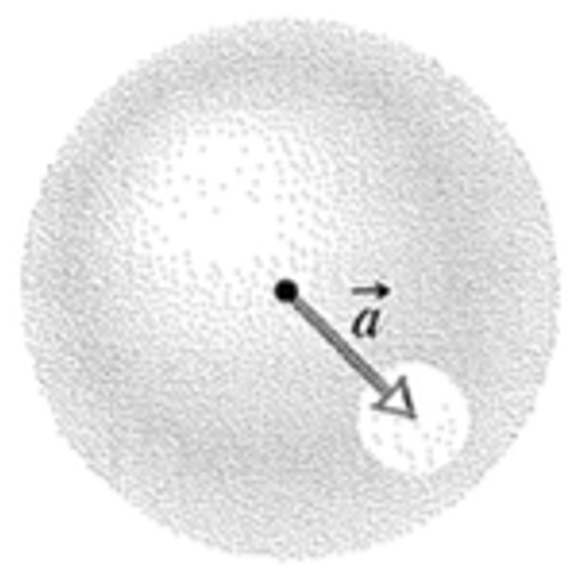
\includegraphics[width=0.20\textwidth]{./images/problems/lect02_spherical_charge_distribution_with_hole}
    \end{center}
  \end{blockexmplque}

\end{frame}

%
%
%

\begin{frame}{Worked example: Exploiting the superposition principle}

  The charge distribution in case of a uniformly charged solid sphere
  with a cavity is equivalent to that of
  a whole uniformly charged solid sphere of charge density $\rho$
  plus a smaller uniformly charged solid sphere
  of charge density -$\rho$ that fills the void.\\
  \vspace{0.2cm}

  \begin{columns}
    \begin{column}{0.38\textwidth}
      \begin{center}
        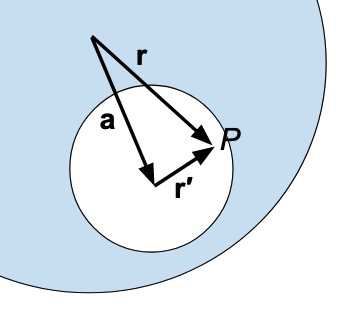
\includegraphics[width=0.95\textwidth]{./images/problems/lect02_sphere_with_cavity_distances_2}
      \end{center}
    \end{column}
    \begin{column}{0.62\textwidth}
      The field produced by each uniformly charged sphere is given.\\
      By superposition, the field at a point $P$ within the cavity
      (at distance $\vec{r}$ from the centre of the larger sphere)
      is given by
      \begin{equation*}
        \vec{E}(\vec{r}) =
        \frac{\rho \vec{r}}{3 \epsilon_0} +
        \frac{(-\rho) \vec{r}^\prime}{3 \epsilon_0} =
           \frac{\rho \vec{r}}{3 \epsilon_0} +
           \frac{(-\rho) (\vec{r} - \vec{a})}{3 \epsilon_0} \Rightarrow
      \end{equation*}
      \begin{equation*}
        \vec{E}(\vec{r}) =
           \frac{\rho \vec{a}}{3 \epsilon_0}
      \end{equation*}
    \end{column}
  \end{columns}

\end{frame}

} %\problemslide


% ------------------------------------------------------------------------------

%
% Worked example :
%

{
\problemslide

\begin{frame}{Worked example: Spherical shell with non-uniform density}

  \begin{blockexmplque}{Question}
    A spherical shell of inner radius $a$ and outer radius $b$ has volume charge
    density $\rho = kr^2$ ($a \le r \le b$), where $k$ is a constant and $r$ is
    the radial distance from the centre of the shell.\\
    Find the magnitude of the electric field $\vec{E}$
    produced by this charge distribution
    at radial distances i) $r<a$, ii) $a \le r < b$, and iii) $b \le r$.
  \end{blockexmplque}

  \vspace{0.2cm}

  Due to the obvious spherical symmetry, the electric field $\vec{E}$
  is a radial vector, and it is
  is going to be a function of only the radial distance $r$.\\

  \vspace{0.2cm}

  We have 3 distinct regions:
  i) $r<a$, ii) $a \le r < b$, and iii) $b \le r$.
  \vspace{0.2cm}

  For the calculation of $\vec{E}$ we will be applying Gauss's theorem:
  \begin{equation*}
    \int_{S} \vec{E} \cdot d\vec{S} =
      \frac{Q_{encl}}{\epsilon_0} =
        \frac{1}{\epsilon_0} \int_{\tau(S)} \rho d\tau
  \end{equation*}

\end{frame}

%
%
%

\begin{frame}{Worked example: Spherical shell with non-uniform density}

  For $r<a$, for {\em any possible} closed surface $S$
  that stays within that region of no charge, Gauss's theorem gives
  \begin{equation*}
    \int_{S} \vec{E} \cdot d\vec{S} = 0
  \end{equation*}
  Since this happens for all surfaces, it can not be the result of an
  accidental cancellation and it has to be that the integrand itself is 0.
  Therefore:
  \begin{equation}
    E (r<a) = 0
  \end{equation}

  \vspace{0.2cm}

  For $a \le r < b$, exploiting the spherical symmetry,
  we will be applying Gauss's theorem
  for a concentric spherical surface $S(r)$ of radius $r$.\\

  \vspace{0.2cm}

  Because both $\vec{E}$ and the surface vector $d\vec{S}$ are collinear,
  and the norm of $\vec{E}$ is constant, everywhere on $S(r)$,
  the flux calculation is simplified:
  \begin{equation*}
    \int_{S(r)} \vec{E} \cdot d\vec{S} =
    \int_{S(r)} E dS =
    E \int_{S(r)} dS =
    E 4\pi r^2
  \end{equation*}

\end{frame}

%
%
%

\begin{frame}{Worked example: Spherical shell with non-uniform density}

  The charge $Q_{enc}$, in the volume $\tau(S)$,
  enclosed by a spherical surface $S(r)$ of radius $r$
  is given by:
  \begin{equation*}
    Q_{enc} =
      \int_{\tau(S)} \rho d\tau =
      \int_{a}^{r} \Big( k u^2 \Big) 4\pi u^2 du =
      4\pi k \int_{a}^{r} u^4 du =
      \frac{4\pi k}{5} u^5 \Big\rvert_{a}^{r} \Rightarrow
  \end{equation*}
  \begin{equation*}
      Q_{enc} =
      \frac{4\pi k}{5} \Big(r^5 - a^5\Big)
  \end{equation*}

  Therefore, Gauss's law can be expressed as:
  \begin{equation*}
    E \cancel{4\pi} r^2 =
     \frac{\cancel{4\pi} k}{5 \epsilon_0} \Big(r^5 - a^5\Big)
  \end{equation*}

  This yields:
  \begin{equation*}
    E (a \le r < b)= \frac{k}{5 \epsilon_0} \Big(r^3 - \frac{a^5}{r^2}\Big)
  \end{equation*}

\end{frame}

%
%
%

\begin{frame}{Worked example: Spherical shell with non-uniform density}

  For $b \le r$, one can apply a similar analysis. In this case,
  $Q_{enc}$ is no longer a function of $r$
  since all spherical surfaces $S(r)$ include all charge.
  From the previous expression for $Q_{enc}$,
  setting $r$ equal to $b$, we have:
  \begin{equation*}
    Q_{enc} =
      \frac{4\pi k}{5} \Big(b^5 - a^5\Big)
  \end{equation*}

  Gauss's law can be expressed as:
  \begin{equation*}
    E \cancel{4\pi} r^2 =
     \frac{\cancel{4\pi} k}{5 \epsilon_0} \Big(b^5 - a^5\Big)
  \end{equation*}

  This yields:
  \begin{equation*}
    E (b \le r)= \frac{k}{5 \epsilon_0} \Big(\frac{b^5 - a^5}{r^2}\Big)
  \end{equation*}

  Summarizing, we found that:
  \begin{equation*}
    \displaystyle
    E =
      \begin{cases}
        0 & \text{ for } r < a\\
        \frac{k}{5 \epsilon_0} \Big(r^3 - \frac{a^5}{r^2}\Big) & \text{ for } a \le r < b\\
        \frac{k}{5 \epsilon_0} \Big(\frac{b^5 - a^5}{r^2}\Big) & \text{ for } b \le r
      \end{cases}
  \end{equation*}

\end{frame}

} %\problemslide

% ------------------------------------------------------------------------------

%
% Worked example :
% H/R Sec 23-9, problem 51 (page 626)
%

{
\problemslide

%
%
%

\begin{frame}{Worked example: Spherical shell and point charge}

  \begin{blockexmplque}{Question}
    The figure below shows
    a nonconducting spherical shell of
    inner radius $a$ and outer radius $b$.
    The shell has (within its thickness) a positive volume charge density
    $\rho(r)$ = $A/r$,
    where $A$ is a constant and $r$ is the distance from the center of the shell.
    In addition, a small ball of charge $q$ is located at that center.
    What value should A have if the electric field in the shell
    ($a < r < b$) is to be uniform?
    \begin{center}
      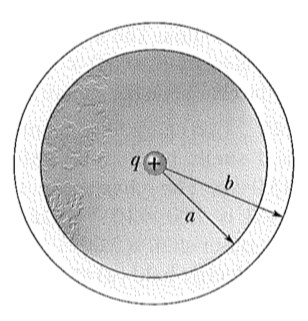
\includegraphics[width=0.30\textwidth]{./images/problems/lect02_thick_spherical_shell_and_central_charge}
    \end{center}
  \end{blockexmplque}

\end{frame}

%
%
%

\begin{frame}{Worked example: Spherical shell and point charge}

  Gauss's law in integral form is:
  \begin{equation*}
  	 \Phi = \frac{Q_{enc}}{\epsilon_0}
  \end{equation*}

  The electric flux $\Phi$ over a closed surface $S$ is defined as:
  \begin{equation*}
  	 \Phi = \oint_{S} \vec{E} \cdot d\vec{S}
  \end{equation*}

  Consider a spherical Gaussian surface with radius $r$, where $a < r < b$.
  Exploiting the spherical symmetry of the problem, we can write:
  \begin{equation*}
  	 \Phi = \oint_{S} E dS = E \oint_{S} dS = E 4\pi r^2
  \end{equation*}

\end{frame}

%
%
%

\begin{frame}{Worked example: Spherical shell and point charge}

  The charge in the volume $\tau(S)$,
  enclosed by the spherical Gaussian surface $S$ with radius $r$,
  is the charge $q$ at the origin and the fraction of the charge of the shell
  that is distributed at radial distances between $a$ and $r$.

  Therefore:
  \begin{equation*}
  	 Q_{enc} = q + \int_{\tau(S)}{\rho d\tau} \Rightarrow
  \end{equation*}

  \begin{equation*}
  	 Q_{enc} = q + \int_{a}^{r} \frac{A}{r^{\prime}} 4\pi {r^{\prime}}^{2} dr^{\prime} \Rightarrow
  	 Q_{enc} = q + 4\pi A \int_{a}^{r} r^{\prime} dr^{\prime} \Rightarrow
  \end{equation*}

  \begin{equation*}
  	 Q_{enc} = q + 4\pi A \frac{{r^{\prime}}^2}{2}\Big\rvert_{a}^{r} \Rightarrow
  	 Q_{enc} = q + 2\pi A (r^2 - a^2)
  \end{equation*}

  Combining the above exressions for $\Phi$ and $Q_{enc}$, we have:

  \begin{equation*}
  	 E 4\pi r^2 = \frac{1}{\epsilon_0} \Big( q + 2\pi A (r^2 - a^2) \Big)
  \end{equation*}

\end{frame}

%
%
%

\begin{frame}{Worked example: Spherical shell and point charge}

  Solving for $E$, we find:
  \begin{equation*}
  	 E = \frac{q + 2\pi A (r^2 - a^2)}{4\pi \epsilon_0 r^2} \Rightarrow
  	 E = \frac{1}{4\pi \epsilon_0 }
      \Big( \frac{q}{r^2} + 2\pi A - \frac{2\pi A a^2}{r^2} \Big)
  \end{equation*}

  The requirement that $E$ is uniform in the shell, implies that:
  \begin{equation*}
      \frac{q}{r^2} - \frac{2\pi A a^2}{r^2} = 0
  \end{equation*}

  Therefore:
  \begin{equation*}
      A = \frac{q}{2\pi a^2}
  \end{equation*}

\end{frame}

} %\problemslide

% ------------------------------------------------------------------------------

%
% Worked example :
% H/R, ch. 23, page 626, question 54
%

{
\problemslide

%
%
%

\begin{frame}{Worked example: Two uniformly charged spheres}

  \begin{blockexmplque}{Question}
    The figure below shows, in cross section, two solid spheres with uniformly
  	distributed charge throughout their volumes. Each has radius R.
  	Point P lies on a line connecting the centres of the spheres, at radial distance
  	R/2.00 from the centre of sphere 1.
  	If the net electric field at point P is zero, what is the ratio $q_2$/$q_1$
  	of the total charges?
    \begin{center}
      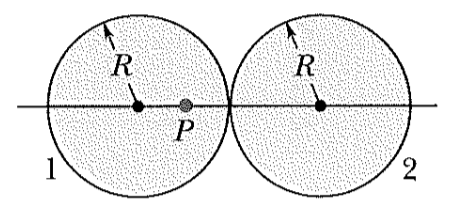
\includegraphics[width=0.60\textwidth]{./images/problems/lect02_2_charged_spheres}
    \end{center}
  \end{blockexmplque}

\end{frame}

%
%
%

\begin{frame}{Worked example: Two uniformly charged spheres}

  The electric field inside and outside a uniformly charged, nonconductive,
  solid sphere of radius $R$ was calculated earlier in this Lecture.\\
  \vspace{0.1cm}
  The results are summarised below:

  {\bf For $r < R$:}
  \begin{equation*}
     E(r) = \frac{Q \frac{r^3}{R^3}}{4 \pi \epsilon_0 r^2} =
      \frac{Q}{4 \pi \epsilon_0 R^3} r
  \end{equation*}

  {\bf For $r \ge R$:}
  \begin{equation*}
     E(r) = \frac{Q}{4 \pi \epsilon_0 r^2}
  \end{equation*}

  \vspace{0.1cm}

  The electric field $\vec{E}$ at point P is the superposition of 2 fields:
  the field $\vec{E}_1$ because of the presence of sphere 1 and
  the field $\vec{E}_2$ because of the presense of sphere 2:
  \begin{equation*}
  	 \vec{E}(P) = \vec{E}_1(P) + \vec{E}_2(P)
  \end{equation*}

\end{frame}

%
%
%

\begin{frame}{Worked example: Two uniformly charged spheres}

  Applying our previous result for the electric field:
  \begin{equation*}
  	\vec{E}_1(P) = \Big\{ \frac{Q}{4 \pi \epsilon_0 R^3} r \Big\} \hat{x} \xRightarrow{Q=q_1, \; r = R/2}
  	\vec{E}_1(P) = \Big\{ \frac{q_1/2}{4 \pi \epsilon_0 R^2} \Big\} \hat{x}
  \end{equation*}

  % \begin{equation*}
  % 	\vec{E}_1(P) = \Big\{ \frac{Q}{4 \pi \epsilon_0 R^3} r \Big\} \hat{x} \xRightarrow{Q=q_1, \; r = R/2}
  % 	\vec{E}_1(P) = \Big\{ \frac{q_1}{4 \pi \epsilon_0 R^3} \frac{R}{2} \Big\} \hat{x} \Rightarrow
  % \end{equation*}
  % \begin{equation*}
  % 	\vec{E}_1(P) = \Big\{ \frac{q_1/2}{4 \pi \epsilon_0 R^2} \Big\} \hat{x}
  % \end{equation*}

  and:
  \begin{equation*}
  	\vec{E}_2(P) = \Big\{ \frac{Q}{4 \pi \epsilon_0 r^2} \Big\} (-\hat{x}) \xRightarrow{Q=q_2, \; r = R+R/2 = 3R/2}
  	\vec{E}_2(P) = - \Big\{ \frac{4q_2/9}{4 \pi \epsilon_0 R^2} \Big\} \hat{x}
  \end{equation*}

  % \begin{equation*}
  % 	\vec{E}_2(P) = \Big\{ \frac{Q}{4 \pi \epsilon_0 r^2} \Big\} (-\hat{x}) \xRightarrow{Q=q_2, \; r = R+R/2 = 3R/2}
  % 	\vec{E}_2(P) = - \Big\{ \frac{q_2}{4 \pi \epsilon_0 (3R/2)^2} \Big\} \hat{x} \Rightarrow
  % \end{equation*}
  % \begin{equation*}
  % 	\vec{E}_2(P) = - \Big\{ \frac{4q_2/9}{4 \pi \epsilon_0 R^2} \Big\} \hat{x}
  % \end{equation*}

  Therefore, the total field is:
  \begin{equation*}
    \vec{E}(P) = \frac{1}{4 \pi \epsilon_0 R^2} (\frac{q_1}{2} - \frac{4q_2}{9}) \hat{x}
  \end{equation*}

  If E(P)=0, then:
  \begin{equation*}
  	\frac{q_1}{2} - \frac{4q_2}{9} = 0 \Rightarrow
    \frac{q_2}{q_1} = \frac{9}{8} \Rightarrow
  	\frac{q_2}{q_1} = 1.125
  \end{equation*}

\end{frame}


} %\problemslide

% ------------------------------------------------------------------------------


%
% Worked example :
% H/R Sec 23-9, problem 50 (page 625)
%

{
\problemslide

%
%
%

\begin{frame}{Worked example: Two spherical shells}

  \begin{blockexmplque}{Question}
    The figure on the left shows
    two nonconducting spherical shells fixed in place on an x axis.
    Shell 1 has uniform surface charge density +4.0 $\mu$C/m$^{2}$
    on its outer surface and radius 0.50 cm, and
    shell 2 has uniform surface charge density -2.0 $\mu$C/m$^{2}$
    on its outer surface and radius 2.0 cm. The shell centres are separated
    by a distance $L$ = 6.0 cm.
    Other than at $x = \infty$,
    where on the x axis is the net electric field equal to zero?
    \begin{center}
      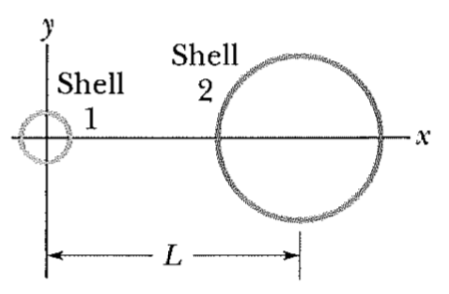
\includegraphics[width=0.40\textwidth]{./images/problems/lect02_2_charged_spherical_shells}
    \end{center}
  \end{blockexmplque}

\end{frame}

%
%
%

\begin{frame}{Worked example: Two spherical shells}

  Consider Gauss's law in its integral form:
  \begin{equation*}
  	 \oint_{S} \vec{E} \cdot d\vec{S} = \frac{Q_{enc}}{\epsilon_0}
  \end{equation*}
  Exploiting the symmetry of a system with charge $Q$ distributed
  uniformly on a spherical, nonconducting shell or radius $R$
  centred at the origin of the coordinate system,
  we can easily calculate the electric field:
  \begin{itemize}
  \item
  For $r < R$, the enclosed charge is 0 and from the symmetry of the problem we
  deduce that $\vec{E}(r) = 0$.
  \item
  For $r \ge R$, all charge Q is enclosed, and the electric field can
  be written (as if we had a point charge at the origin)
  as $\vec{E}(r) = \frac{Q}{4\pi\epsilon_0 r^2} \hat{r}$.\\
  \end{itemize}

  \vspace{0.2cm}
  The electric field $\vec{E}$ produced by the two spherical shells 1 and 2
  is given superposition principle:
  \begin{equation*}
    \vec{E} = \vec{E}_1 + \vec{E}_2
  \end{equation*}
  where $\vec{E}_1$ ($\vec{E}_2$) is the field of sphere 1 (2).\\

\end{frame}

%
%
%

\begin{frame}{Worked example: Two spherical shells}

  The field produced by each shell is pointing radially in (as in the case of
  the negatively charged shell 2) or out (as in the case of the positively
  charged shell 1). Therefore, for all points on the x axis,
  $\vec{E}_1$ and $\vec{E}_2$ point along $\pm \hat{x}$.\\

  \vspace{0.3cm}
  Within shell 1, $\vec{E}_1 = 0$, and within shell 2, $\vec{E}_2 = 0$.
  Therefore, within the shells, the net electric field $\vec{E}_1 + \vec{E}_2$
  cannot be zero there.\\

  \vspace{0.3cm}

  For all x values between the shells ($R_1 < x < L-R_2$),
  the fields $\vec{E}_1$ and $\vec{E}_2$ point in the same direction
  and, therefore, the net electric field $\vec{E}_1 + \vec{E}_2$
  cannot be zero there.\\

  \vspace{0.3cm}

  The charge contained by shells 1 and 2 can be calculated as follows:

  \begin{equation*}
  	 Q_1 = 4\pi R_{1}^{2} \sigma_{1}
         = 4\pi (5\times 10^{-3} \; m)^{2} (4 \times 10^{-6} \; C/m^2)
         = 4\pi \times 10^{-10} \; C
  \end{equation*}
  \begin{equation*}
  	|Q_2| = 4\pi R_{2}^{2} |\sigma_{2}|
          = 4\pi (2\times 10^{-2} \; m)^{2} (2 \times 10^{-6} \; C/m^2)
          = 8 \times 4\pi \times 10^{-10} \; C
  \end{equation*}

\end{frame}

%
%
%

\begin{frame}{Worked example: Two spherical shells}

  Since $|Q_2| > Q_1$,
  $|\vec{E}_2|>|\vec{E}_1|$ for all values of $x > L + R_2$
  (closer to shell 2 than to shell 1). Therefore,
  the net field $\vec{E}_1 + \vec{E}_2$ cannot be zero there.\\

  \vspace{0.3cm}

  Following from the above, the only range of x values where
  the net field $\vec{E}_1 + \vec{E}_2$ can be zero, is $x < -R_1$.
  In that range,  $\vec{E}_1$ and $\vec{E}_2$ have opposite directions,
  and magnitudes given by:

  \begin{equation*}
  	 E_1 = \frac{1}{4\pi \epsilon_0} \frac{Q_1}{|x|^2} \xRightarrow{4\pi R_{1}^{2} \sigma_{1}}
  	 E_1 = \frac{R_{1}^{2} \sigma_{1}}{\epsilon_0} \frac{1}{|x|^2}
  \end{equation*}

  \begin{equation*}
  	 E_2 = \frac{1}{4\pi \epsilon_0} \frac{|Q_2|}{(L+|x|)^2} \xRightarrow{|Q_2|=4\pi R_{2}^{2} |\sigma_{2}|}
  	 E_2 = \frac{R_{2}^{2} |\sigma_{2}|}{\epsilon_0} \frac{1}{(L+|x|)^2}
  \end{equation*}

  The requirement that the net electric field is zero, implies that:
  \begin{equation*}
  	 E_1 = E_2
  \end{equation*}

\end{frame}

%
%
%

\begin{frame}{Worked example: Two spherical shells}

  Therefore:
  \begin{equation*}
    \frac{R_{1}^{2} \sigma_{1}}{\epsilon_0} \frac{1}{|x|^2} =
    \frac{R_{2}^{2} |\sigma_{2}|}{\epsilon_0} \frac{1}{(L+|x|)^2} \Rightarrow
  \end{equation*}

  \begin{equation*}
    \Big( \frac{L+|x|}{|x|} \Big)^2 = \frac{R_{2}^{2} |\sigma_{2}|}{R_{1}^{2} \sigma_{1}} \Rightarrow
    \frac{L}{|x|} + 1  = \frac{R_{2}}{R_{1}} \sqrt{\frac{|\sigma_{2}|}{\sigma_{1}}} \Rightarrow
  \end{equation*}

  \begin{equation*}
    |x| = \frac{L}{ \frac{R_{2}}{R_{1}} \sqrt{\frac{|\sigma_{2}|}{\sigma_{1}}} - 1} \Rightarrow
  \end{equation*}

  \begin{equation*}
    |x| = \frac{6\; cm}{ \frac{2.0}{0.5} \sqrt{\frac{2}{4}} - 1}
        = \frac{6\; cm}{ \frac{4}{\sqrt{2}} - 1} \approx 3.28 \; cm
    \Rightarrow
    x \approx -3.28 \; cm
  \end{equation*}

\end{frame}

} %\problemslide

% ------------------------------------------------------------------------------

%
% Worked example :
%

{
\problemslide

\begin{frame}{Worked example: Electric field of two charged sheets}

  \begin{blockexmplque}{Question}
       Two uniform infinite sheets of electric charge densities
       $+\sigma$ and $-\sigma$ intersect at a right angle.
       Find the magnitude and direction of the electric field everywhere
       and sketch the electric field lines.
  \end{blockexmplque}

  The magnitude of the electric field caused by a single, infinite sheet
  of uniform charge density $\sigma$ is given by:
  \begin{equation*}
     E = \frac{\sigma}{2\epsilon_0}
  \end{equation*}

  The direction of the field is perpendicular to the sheet and it is pointing
  towards (away from) the sheet, if it is negatively (positively) charged.

  The field in the problem of two uniform infinite sheets
  can be obtained by invoking the superposition principle
  and superimposing undisturbed
  \begin{itemize}
  \item
  the field $\vec{E_(+)}$
  of an infinite sheet of uniform charge density $+\sigma$, and
  \item
  the field $\vec{E_(-)}$
  of an infinite sheet of uniform charge density $-\sigma$.
  \end{itemize}

\end{frame}

%
%
%

\begin{frame}{Worked example: Electric field of two charged sheets}

  The magnitude of the combined field ($\vec{E}$) is:
  \begin{equation*}
     E = \sqrt{E_(+)^2 + E_(-)^2}
       = \sqrt{\Big( \frac{+\sigma}{2\epsilon_0} \Big)^2 +
               \Big( \frac{-\sigma}{2\epsilon_0} \Big)^2} \Rightarrow
     E = \frac{\sqrt{2}\sigma}{2\epsilon_0}
  \end{equation*}
  The field lines are sketched below:
  \begin{figure}[htb]
    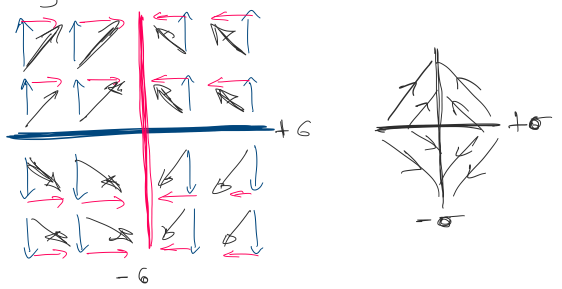
\includegraphics[width=0.8\linewidth]{./images/problems/lect02_field_lines_of_2_charged_sheets}
  \end{figure}


\end{frame}

} %\problemslide

% ------------------------------------------------------------------------------

{
\programmingslide

%
%
%

\begin{frame}{PHYS201 scientific programming task for Lecture \thislecture}

{\small

If you did the previous task, you already have a program to calculate the
electric field (in 2-D) for an arbitrary distribution of discrete charges.\\
\vspace{0.2cm}

Generalize your previous program:
\begin{itemize}
{
  \item Move from a 2-D to a {\bf 3-D calculation}.
  \item Add an option to {\bf specify a continuous distribution of charge}
        (i.e. work with a user-defined charge density function $\rho(\vec{r})$)
}
\end{itemize}

\vspace{0.2cm}
What you will be doing, is to perform the following numerical integration:
\begin{equation*}
   \vec{E}(\vec{r}) = \frac{1}{4\pi\epsilon_0} \int_{\tau}
      d\tau^{\prime} \frac{\rho({\pvec{r}'})}{|\vec{r}-\pvec{r}'|^{3}} (\vec{r}-\pvec{r}')
\end{equation*}

\vspace{0.3cm}

Can you test Gauss' law numerically?

}
\end{frame}

%
%
%

\begin{frame}{PHYS201 scientific programming task for Lecture \thislecture}

{\small

As an example, use the following charge density in spherical coordinates:
\begin{equation*}
   \rho =
     \begin{cases}
       \frac{\rho_0}{(r/r_0)^2} e^{-r/r_0} cos^2\phi, & \text{if $r < 5 r_0$} \\
       & \\
       0, \text{otherwise}
     \end{cases}
\end{equation*}
where $\rho_0$ = 0.16 C/m$^{3}$ and r$_0$ = 10 cm.\\
%
% at r = 5 *r0, the charge contained is 6.24 * \rho_0 * ro^3
% 0.16 is 1/6.24
%

\vspace{0.2cm}
Calculate numerically the amount of charge Q enclosed in a sphere of radius r, as a function or r:\\
\begin{equation*}
  Q(r) = \int_{0}^{r} \int_{4\pi} d\tau \rho(\vec{r^\prime})
\end{equation*}

\vspace{0.2cm}
Confirm that your distribution plateaus to a value of $Q_{tot}$ for
r $>5r_0$, as the sphere encloses all regions of non-zero charge density.
What is the value of $Q_{tot}$?\\

\vspace{0.2cm}
Calculate the electric flux through the surface of a sphere with radius r = 5$r_0$
and confirm that:
\begin{equation*}
  \epsilon_0 \oint \vec{E} \cdot d\vec{S} = Q_{tot}
\end{equation*}
}

\end{frame}

} % programming
